% ─── Chapter 5: ROM & Hyper-Reduction ──────────────────────────────────────────

% ==========================================
% Frame 1: Why ROM? (Motivation)
% ==========================================
\begin{frame}{Why ROM? (Motivation)}
  \small
  \begin{columns}[T]
    \begin{column}{0.55\textwidth}
      \begin{block}{The Full-Order Bottleneck}
        \begin{itemize}
          \item High-fidelity Full Order Model (FOM) has $N = 6,564$ DOFs.
          \item Online matrix assembly scales with mesh size $\mathcal{O}(N)$.
          \item Solves are too slow for real-time interactivity.
        \end{itemize}
      \end{block}
      \vspace{0.1cm}
      \begin{block}{Need for Interactivity}
        \begin{itemize}
          \item Interactive client-side web browser execution.
          \item Must bypass the full-order assembly bottleneck.
          \item Target frame rate: 20--60 FPS ($<1.5\text{ ms}$ solve time).
        \end{itemize}
      \end{block}
    \end{column}
    \begin{column}{0.42\textwidth}
      \centering
      \begin{alertblock}{Interactive Budget}
        \centering
        \bfseries
        Online Solve Time: \Large $< 1.5\text{ ms}$
      \end{alertblock}
      
      \vspace{0.25cm}
      \centering
      \begin{tikzpicture}[scale=0.72, every node/.style={transform shape}]
        % Equation parts: K_r = Phi^T * K * Phi
        
        % K_r (small red square)
        \draw[fill=cnamred!20, draw=cnamred, thick] (0, 0.75) rectangle (0.30, 1.05);
        \node[above] at (0.15, 1.05) {$\mathbf{K}_r$};
        \node[below, font=\tiny] at (0.15, 0.75) {\bfseries $r \times r$};
        
        % =
        \node at (0.7, 0.9) {\large $=$};
        
        % \Phi^T (horizontal blue rectangle)
        \draw[fill=blue!10, draw=blue!60, thick] (1.0, 0.75) rectangle (2.8, 1.05);
        \node[above] at (1.9, 1.05) {$\boldsymbol{\Phi}^T$};
        \node[below, font=\tiny] at (1.9, 0.75) {\bfseries $r \times N$};
        
        % K (large gray square)
        \draw[fill=gray!20, draw=gray!70, thick] (3.1, 0) rectangle (4.9, 1.8) node[midway, font=\small] {$\mathbf{K}$};
        \node[below, font=\tiny] at (4.0, 0) {\bfseries $N \times N$};
        
        % \Phi (vertical blue rectangle)
        \draw[fill=blue!10, draw=blue!60, thick] (5.2, 0) rectangle (5.5, 1.8);
        \node[above] at (5.35, 1.8) {$\boldsymbol{\Phi}$};
        \node[below, font=\tiny] at (5.35, 0) {\bfseries $N \times r$};
      \end{tikzpicture}
      
      \vspace{0.15cm}
      \footnotesize
      \begin{tabular}{rcc}
        \toprule
         & \textbf{FOM} & \textbf{ROM} \\
        \midrule
        \textbf{Dimension} & $N = 6,564$ & $r = 15$ \\
        \textbf{Matrix entries} & $\approx 43\text{M}$ & $\mathbf{225}$ \\
        \bottomrule
      \end{tabular}
    \end{column}
  \end{columns}
\end{frame}

% ==========================================
% Frame 2: What Do We Need to Achieve It? (The Steps)
% ==========================================
\begin{frame}{What Do We Need to Achieve It? (The Steps)}
  \small
  \vspace{-0.15cm}
  \begin{columns}[T]
    \begin{column}{0.50\textwidth}
      \begin{block}{Offline Phase (Preparation)}
        \begin{itemize}
          \setlength{\itemsep}{0.06cm}
          \item \textbf{1. Pullback}: Fix static reference mesh $\hat{\Omega}$.
          \item \textbf{2. Snapshots}: Generate state vectors across $\mathcal{D}$.
          \item \textbf{3. SVD / POD}: Extract optimal basis $\boldsymbol{\Phi}$.
        \end{itemize}
      \end{block}
      \vspace{0.08cm}
      \begin{block}{Online Phase (Real-Time Interactivity)}
        \begin{itemize}
          \setlength{\itemsep}{0.06cm}
          \item \textbf{4. Galerkin ROM}: Project to $r$ DOFs ($r \ll N$).
          \item \textbf{5. ECSW}: Hyper-reduction for sparse assembly.
        \end{itemize}
      \end{block}
    \end{column}
    
    \begin{column}{0.48\textwidth}
      \centering
      \scalebox{0.74}{
      \begin{tikzpicture}[
          node distance=0.42cm,
          stepbox/.style={draw=cnamred, fill=cnamlightbg, thick, rounded corners, minimum width=3.8cm, minimum height=0.52cm, align=center, font=\scriptsize},
          branchbox/.style={draw=cnamdark, fill=cnamlightbg, thick, rounded corners, minimum width=2.4cm, minimum height=0.90cm, align=center, font=\tiny},
          arrow/.style={thick,->,>=stealth, cnamred}
      ]
          % --- OFFLINE/ONLINE DIVIDER & LABELS ---
          \draw[dashed, gray!40, thick] (-2.6, -2.2) -- (2.6, -2.2);
          \node[anchor=east, font=\tiny\bfseries, color=gray] at (-2.7, -1.0) {OFFLINE};
          \node[anchor=east, font=\tiny\bfseries, color=cnamred] at (-2.7, -3.5) {ONLINE};
          
          % Nodes
          \node[stepbox] (s1) at (0, 0) {1. Reference Pullback Mapping};
          \node[stepbox, below=of s1] (s2) {2. Snapshot Collection};
          \node[stepbox, below=of s2] (s3) {3. SVD / POD Basis Construction};
          
          % Parallel Online Branches
          \node[branchbox] (gal4) at (-1.5, -3.2) {\textbf{Galerkin ROM Path} \\ Full Assembly \\ (no hyper-reduction)};
          \node[branchbox, below=0.3cm of gal4] (gal5) {\textbf{Reduced Solve} \\ (Newmark-$\beta$ in $r\ll N$)};
          
          \node[branchbox, draw=orange!70] (ecsw4) at (1.5, -3.2) {\textbf{ECSW ROM Path} \\ \textbf{Sparse Assembly} \\ (Hyper-reduced)};
          \node[branchbox, draw=orange!70, below=0.3cm of ecsw4] (ecsw5) {\textbf{Reduced Solve} \\ (Newmark-$\beta$ in $r\ll N$)};
          
          % Arrows
          \draw[arrow] (s1) -- (s2);
          \draw[arrow] (s2) -- (s3);
          
          % Clean split below the divider line
          \draw[thick, cnamred] (s3.south) -- (0, -2.4);
          \draw[arrow] (0, -2.4) -| (gal4.north);
          \draw[arrow] (0, -2.4) -| (ecsw4.north);
          
          % Connections within branches
          \draw[arrow] (gal4) -- (gal5);
          \draw[arrow] (ecsw4) -- (ecsw5);
      \end{tikzpicture}
      }
    \end{column}
  \end{columns}
\end{frame}

% ==========================================
% Frame 3: Step 1: Reference Pullback Mapping
% ==========================================
\begin{frame}{Step 1: Reference Pullback Mapping}
  \centering
  \vspace{-0.1cm}

  {\small\textbf{The Motivation}: Why does shape-parametric ROM require a reference domain?}
  \par\vspace{0.3cm}

  \begin{columns}[T]
    \begin{column}{0.48\textwidth}
      \begin{block}{Physical Domain $\Omega(\boldsymbol{\mu})$}
        \footnotesize
        \textbf{Deforming Coordinates}:
        \begin{itemize}
          \setlength{\itemsep}{0.1cm}
          \item Mesh shifts with parameter $\boldsymbol{\mu}$.
          \item Snapshots live in different spaces.
          \item \textcolor{cnamred}{\textbf{Cannot build a global POD basis}}.
        \end{itemize}
      \end{block}
    \end{column}

    \begin{column}{0.48\textwidth}
      \begin{exampleblock}{Reference Domain $\hat{\Omega}$}
        \footnotesize
        \textbf{Invariant Coordinate Space}:
        \begin{itemize}
          \setlength{\itemsep}{0.1cm}
          \item Static mesh: state $\vect{U} \in \mathbb{R}^N$ for all $\boldsymbol{\mu}$.
          \item Snapshots share the same coordinates.
          \item \textcolor{teal!80!black}{\textbf{Enables a single POD basis $\boldsymbol{\Phi}$}}.
        \end{itemize}
      \end{exampleblock}
    \end{column}
  \end{columns}

  \vspace{0.3cm}

  \begin{alertblock}{Core Takeaway}
    \centering\footnotesize
    Geometry variations are absorbed into mapping weights $J(\boldsymbol{\mu})$, keeping the state vector space invariant for model reduction.
  \end{alertblock}
\end{frame}

% ==========================================
% Frame 4: Step 2: Snapshot Collection
% ==========================================
\begin{frame}{Step 2: Snapshot Collection (Data Generation)}
  \small
  \begin{columns}[T]
    \begin{column}{0.55\textwidth}
      \begin{block}{What is a Snapshot?}
        \begin{itemize}
          \item A high-fidelity state vector representing the structural displacement field $\vect{U}(t) \in \mathbb{R}^N$ on the reference mesh $\hat{\Omega}$.
        \end{itemize}
      \end{block}
      \begin{block}{Snapshot Matrix}
        \begin{itemize}
          \item Compile all state vectors into snapshot matrix:
          \[
            \mathbf{S}_u = [\vect{u}_1, \vect{u}_2, \dots, \vect{u}_d] \in \mathbb{R}^{N \times d}
          \]
        \end{itemize}
      \end{block}
    \end{column}
    \begin{column}{0.42\textwidth}
      \begin{exampleblock}{Representative Load Cases}
        FOM simulations are run offline across representative configurations to capture dominant physics:
        \begin{itemize}
          \item Tip bending load
          \item Mid-span bending load
          \item Analytical axial tension
        \end{itemize}
      \end{exampleblock}
    \end{column}
  \end{columns}
\end{frame}

% ==========================================
% Frame 5: Step 3: SVD / POD Basis Construction
% ==========================================
\begin{frame}{Step 3: SVD / POD Basis Construction}
  \small
  \begin{columns}[T]
    \begin{column}{0.51\textwidth}
      \textbf{Dimensionality Reduction}:
      \begin{itemize}
        \setlength{\itemsep}{0.1cm}
        \item Perform Singular Value Decomposition (SVD):
        \[
          \mathbf{S}_u = \mathbf{U} \boldsymbol{\Sigma} \mathbf{V}^T, \quad \boldsymbol{\Sigma} = \operatorname{diag}(\sigma_1, \dots, \sigma_d)
        \]
        \item Keep the first $r$ dominant modes of $\mathbf{U}$ to form the Reduced Basis matrix $\boldsymbol{\Phi} \in \mathbb{R}^{N \times r}$:
        \[
          \vect{U}(t) \approx \boldsymbol{\Phi}\,\vect{q}(t), \quad r\ll N
        \]
      \end{itemize}
    \end{column}
    \begin{column}{0.46\textwidth}
      \begin{block}{Cumulative Energy \& Error}
        \scriptsize
        \centering
        \[
          \eta(r) = \frac{\sum_{i=1}^{r} \sigma_i^2}{\sum_{j=1}^{d} \sigma_j^2}, \quad \epsilon(r) = \sqrt{1 - \eta(r)}
        \]
        \vspace{-0.15cm}
        \begin{tabular}{lcc}
          \toprule
          Modes $r$ & Energy $\eta(r)$ & Error $\epsilon(r)$ \\
          \midrule
          1  & 99.945\% & 2.34\% \\
          5  & 99.992\% & 0.89\% \\
          10 & 99.999\% & 0.11\% \\
          \bottomrule
        \end{tabular}
        \par\vspace{0.08cm}
        Captures $>99.99\%$ energy with just $r=10$ modes.
      \end{block}
    \end{column}
  \end{columns}
\end{frame}

% ==========================================
% Frame 6: Step 4: Galerkin Projection vs. ECSW Hyper-reduction
% ==========================================
\begin{frame}{Step 4: Galerkin Projection vs. ECSW Hyper-reduction}
  \small
  \begin{columns}[T]
    \begin{column}{0.48\textwidth}
      \begin{block}{Galerkin Projection ($r \times r$)}
        \footnotesize
        \[
          \mat{M}_r\ddot{\vect{q}} + \mat{C}_r\dot{\vect{q}} + \mat{K}_r(\boldsymbol{\mu})\vect{q} = \vect{F}_r(t)
        \]
        \alert{Assembly Bottleneck}: Requires assembling the full matrix $\hat{\mat{K}}(\boldsymbol{\mu}) \in \mathbb{R}^{N \times N}$ online. No online speedup ($0.92\times$).
      \end{block}
      
      \vspace{0.1cm}
      \centering
      \begin{tikzpicture}[scale=0.75, every node/.style={transform shape}]
        % Mesh (All active)
        \foreach \x in {0,...,3} {
          \foreach \y in {0,...,3} {
            \draw[fill=cnamred!20, draw=cnamred!70] (\x*0.4, \y*0.4) rectangle (\x*0.4+0.35, \y*0.4+0.35);
          }
        }
        \node[below, font=\tiny\bfseries] at (0.75, 0) {Mesh (3,200 elements)};
        \node[right, font=\tiny, align=left] at (1.65, 0.8) {\textbf{Evaluate}\\\textbf{ALL} elements};
        
        % Arrow to N x N
        \draw[->, thick, cnamred] (0.75, -0.15) -- (0.75, -0.65);
        
        % Giant Matrix
        \draw[fill=gray!15, draw=gray!60, thick] (0.2, -1.7) rectangle (1.3, -0.8) node[midway, font=\scriptsize] {$\hat{\mat{K}}(\boldsymbol{\mu})$};
        \node[below, font=\tiny] at (0.75, -1.7) {$N \times N$ (Full)};
        
        % Arrow to small matrix
        \draw[->, thick, cnamred] (1.45, -1.25) -- (1.95, -1.25);
        
        % Small Matrix
        \draw[fill=cnamred!15, draw=cnamred, thick] (2.1, -1.5) rectangle (2.6, -1.0) node[midway, font=\tiny] {$\mat{K}_r$};
        \node[below, font=\tiny] at (2.35, -1.5) {$r \times r$};
      \end{tikzpicture}
    \end{column}
    
    \begin{column}{0.48\textwidth}
      \begin{block}{ECSW Hyper-Reduction}
        \footnotesize
        ECSW integrates only over a sparse active subset of elements $\tilde{\Omega} \subset \Omega$:
        \[
          \mat{K}_{r,\text{ECSW}}(\boldsymbol{\mu}) = \sum_{e\in\tilde{\Omega}} w_e\,\boldsymbol{\Phi}_e^T\mat{K}_e(\boldsymbol{\mu})\boldsymbol{\Phi}_e
        \]
        Bypasses the assembly bottleneck, evaluating only $28$ out of $3,200$ elements online.
      \end{block}
      
      \vspace{0.1cm}
      \centering
      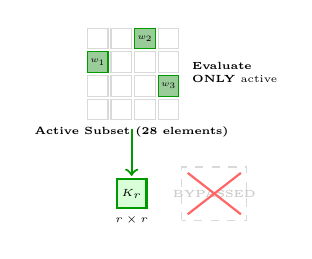
\begin{tikzpicture}[scale=0.75, every node/.style={transform shape}]
        % Mesh (Sparse active)
        \foreach \x in {0,...,3} {
          \foreach \y in {0,...,3} {
            \draw[fill=white, draw=gray!30] (\x*0.4, \y*0.4) rectangle (\x*0.4+0.35, \y*0.4+0.35);
          }
        }
        % Highlighted elements with weights
        \draw[fill=green!50!black!40, draw=green!60!black] (0*0.4, 2*0.4) rectangle (0*0.4+0.35, 2*0.4+0.35) node[midway, font=\tiny\bfseries, scale=0.8] {$w_1$};
        \draw[fill=green!50!black!40, draw=green!60!black] (2*0.4, 3*0.4) rectangle (2*0.4+0.35, 3*0.4+0.35) node[midway, font=\tiny\bfseries, scale=0.8] {$w_2$};
        \draw[fill=green!50!black!40, draw=green!60!black] (3*0.4, 1*0.4) rectangle (3*0.4+0.35, 1*0.4+0.35) node[midway, font=\tiny\bfseries, scale=0.8] {$w_3$};
        
        \node[below, font=\tiny\bfseries] at (0.75, 0) {Active Subset (28 elements)};
        \node[right, font=\tiny, align=left] at (1.65, 0.8) {\textbf{Evaluate}\\\textbf{ONLY} active};
        
        % Arrow directly to small matrix
        \draw[->, thick, green!60!black] (0.75, -0.15) -- (0.75, -0.95);
        
        % Small Matrix
        \draw[fill=green!15, draw=green!60!black, thick] (0.5, -1.5) rectangle (1.0, -1.0) node[midway, font=\tiny] {$\mat{K}_r$};
        \node[below, font=\tiny] at (0.75, -1.5) {$r \times r$};
        % Crossed out giant matrix area (Bypassed)
        \draw[dashed, gray!30] (1.6, -1.7) rectangle (2.7, -0.8);
        \node[gray!40, font=\tiny\bfseries] at (2.15, -1.25) {BYPASSED};
        \draw[red!60, thick] (1.7, -0.9) -- (2.6, -1.6);
        \draw[red!60, thick] (1.7, -1.6) -- (2.6, -0.9);
      \end{tikzpicture}
    \end{column}
  \end{columns}
\end{frame}

% ==========================================
% Frame 7: Step 5: Real-Time Solver & Benchmarks
% ==========================================
\begin{frame}{Step 5: Real-Time Solver \& Benchmarks}
  \small
  \begin{columns}[c]
    \begin{column}{0.48\textwidth}
      \begin{block}{Quantitative Comparative Performance}
        \centering\footnotesize
        \resizebox{\textwidth}{!}{%
        \begin{tabular}{lcccc}
          \toprule
          \textbf{Solver Strategy} & \textbf{Cells} & \textbf{$L_2$ Error} & \textbf{Time} & \textbf{Speedup} \\
          \midrule
          Full Order (FOM)        & 3,200 & Baseline & 142.1 ms & $1.0\times$ \\
          Galerkin ROM            & 3,200 & $0.012\%$ & 154.5 ms & $0.92\times$ \\
          \textbf{ECSW ROM}       & \textbf{28}  & \textbf{0.054\%} & \textbf{2.2 ms} & \textbf{64.5$\times$} \\
          \bottomrule
        \end{tabular}%
        }
      \end{block}
    \end{column}
    
    \begin{column}{0.48\textwidth}
      \centering
      \scalebox{0.6}{
      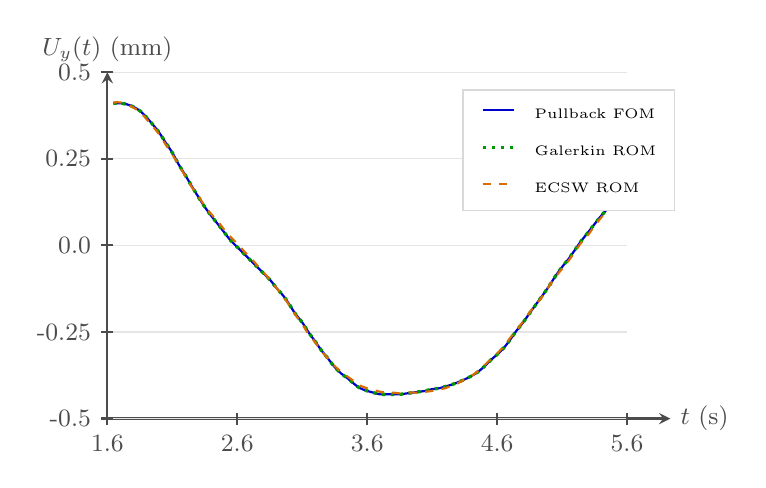
\begin{tikzpicture}[scale=1.1, >=stealth]
        % Axes
        \draw[->, thick, black!70] (0,0) -- (6.5,0) node[right, font=\small] {$t$ (s)};
        \draw[->, thick, black!70] (0,0) -- (0,4.0) node[above, font=\small] {$U_y(t)$ (mm)};
        
        % Y Grid lines and Ticks
        \foreach \y/\label in {0.0/-0.5, 1.0/-0.25, 2.0/0.0, 3.0/0.25, 4.0/0.5} {
            \draw[gray!20, thin] (0, \y) -- (6.0, \y);
            \draw[black!70, thick] (2pt, \y) -- (-2pt, \y) node[left, font=\small] {\label};
        }
        % X Ticks
        \foreach \x/\label in {0/1.6, 1.5/2.6, 3.0/3.6, 4.5/4.6, 6.0/5.6} {
            \draw[black!70, thick] (\x, 2pt) -- (\x, -2pt) node[below, font=\small] {\label};
        }
        
        % Plot Full Pullback FOM (solid blue line)
        \draw[blue!80!black, thick, smooth] plot coordinates {
            (0.07,3.64) (0.15,3.64) (0.22,3.63) (0.30,3.60) (0.38,3.55) (0.45,3.48) (0.52,3.40) (0.60,3.30) (0.67,3.19) (0.75,3.07) (0.82,2.94) (0.90,2.81) (0.97,2.69) (1.05,2.56) (1.12,2.45) (1.20,2.34) (1.28,2.24) (1.35,2.15) (1.42,2.06) (1.50,1.98) (1.57,1.91) (1.65,1.83) (1.72,1.76) (1.80,1.68) (1.88,1.60) (1.95,1.51) (2.03,1.42) (2.10,1.32) (2.17,1.21) (2.25,1.11) (2.32,1.00) (2.40,0.89) (2.47,0.79) (2.55,0.69) (2.62,0.60) (2.70,0.52) (2.78,0.46) (2.85,0.40) (2.92,0.35) (3.00,0.32) (3.07,0.30) (3.15,0.28) (3.22,0.28) (3.30,0.28) (3.38,0.28) (3.45,0.29) (3.53,0.30) (3.60,0.31) (3.67,0.32) (3.75,0.34) (3.83,0.35) (3.90,0.37) (3.97,0.39) (4.05,0.42) (4.12,0.45) (4.20,0.49) (4.28,0.54) (4.35,0.60) (4.42,0.67) (4.50,0.74) (4.58,0.82) (4.65,0.91) (4.72,1.01) (4.80,1.11) (4.87,1.21) (4.95,1.32) (5.03,1.43) (5.10,1.53) (5.17,1.64) (5.25,1.75) (5.33,1.85) (5.40,1.95) (5.47,2.05) (5.55,2.15) (5.62,2.24) (5.70,2.34) (5.78,2.43) (5.85,2.52) (5.92,2.62) (6.00,2.71)
        };
        
        % Plot Galerkin ROM (dotted green line, almost identical to FOM)
        \draw[green!60!black, dotted, very thick, smooth] plot coordinates {
            (0.07,3.64) (0.15,3.64) (0.22,3.63) (0.30,3.60) (0.38,3.55) (0.45,3.48) (0.52,3.40) (0.60,3.30) (0.67,3.19) (0.75,3.07) (0.82,2.94) (0.90,2.81) (0.97,2.69) (1.05,2.56) (1.12,2.45) (1.20,2.34) (1.28,2.24) (1.35,2.15) (1.42,2.06) (1.50,1.98) (1.57,1.91) (1.65,1.83) (1.72,1.76) (1.80,1.68) (1.88,1.60) (1.95,1.51) (2.03,1.42) (2.10,1.32) (2.17,1.21) (2.25,1.11) (2.32,1.00) (2.40,0.89) (2.47,0.79) (2.55,0.69) (2.62,0.60) (2.70,0.52) (2.78,0.46) (2.85,0.40) (2.92,0.35) (3.00,0.32) (3.07,0.30) (3.15,0.28) (3.22,0.28) (3.30,0.28) (3.38,0.28) (3.45,0.29) (3.53,0.30) (3.60,0.31) (3.67,0.32) (3.75,0.34) (3.83,0.35) (3.90,0.37) (3.97,0.39) (4.05,0.42) (4.12,0.45) (4.20,0.49) (4.28,0.54) (4.35,0.60) (4.42,0.67) (4.50,0.74) (4.58,0.82) (4.65,0.91) (4.72,1.01) (4.80,1.11) (4.87,1.21) (4.95,1.32) (5.03,1.43) (5.10,1.53) (5.17,1.64) (5.25,1.75) (5.33,1.85) (5.40,1.95) (5.47,2.05) (5.55,2.15) (5.62,2.24) (5.70,2.34) (5.78,2.43) (5.85,2.52) (5.92,2.62) (6.00,2.71)
        };
        
        % Plot ECSW Mapped ROM (dashed orange line)
        \draw[orange!85!black, dashed, thick, smooth] plot coordinates {
            (0.07,3.65) (0.15,3.65) (0.22,3.63) (0.30,3.59) (0.38,3.54) (0.45,3.46) (0.52,3.38) (0.60,3.28) (0.67,3.17) (0.75,3.05) (0.82,2.93) (0.90,2.80) (0.97,2.68) (1.05,2.57) (1.12,2.46) (1.20,2.36) (1.28,2.27) (1.35,2.18) (1.42,2.10) (1.50,2.02) (1.57,1.94) (1.65,1.86) (1.72,1.78) (1.80,1.69) (1.88,1.60) (1.95,1.51) (2.03,1.41) (2.10,1.31) (2.17,1.20) (2.25,1.09) (2.32,0.98) (2.40,0.88) (2.47,0.78) (2.55,0.69) (2.62,0.61) (2.70,0.54) (2.78,0.48) (2.85,0.43) (2.92,0.38) (3.00,0.35) (3.07,0.33) (3.15,0.31) (3.22,0.30) (3.30,0.30) (3.38,0.29) (3.45,0.30) (3.53,0.30) (3.60,0.30) (3.67,0.31) (3.75,0.32) (3.83,0.34) (3.90,0.35) (3.97,0.38) (4.05,0.41) (4.12,0.45) (4.20,0.49) (4.28,0.55) (4.35,0.61) (4.42,0.68) (4.50,0.75) (4.58,0.84) (4.65,0.93) (4.72,1.02) (4.80,1.12) (4.87,1.22) (4.95,1.32) (5.03,1.42) (5.10,1.53) (5.17,1.63) (5.25,1.73) (5.33,1.83) (5.40,1.93) (5.47,2.03) (5.55,2.12) (5.62,2.22) (5.70,2.32) (5.78,2.42) (5.85,2.51) (5.92,2.61) (6.00,2.71)
        };
        
        % Legend (Vertical, top-right)
        \matrix [draw=gray!30, fill=white, at={(4.1, 3.8)}, anchor=north west, font=\tiny, row sep=3pt, ampersand replacement=\&] {
            \node {\tikz[baseline=-0.5ex]{\draw[blue!80!black, thick] (0,0) -- (0.4,0);}}; \& \node {Pullback FOM}; \\
            \node {\tikz[baseline=-0.5ex]{\draw[green!60!black, dotted, very thick] (0,0) -- (0.4,0);}}; \& \node {Galerkin ROM}; \\
            \node {\tikz[baseline=-0.5ex]{\draw[orange!85!black, dashed, thick] (0,0) -- (0.4,0);}}; \& \node {ECSW ROM}; \\
        };
      \end{tikzpicture}
      }
      \\[2pt]
      \scriptsize\centering Tip deflection $U_y(t)$ comparison curves
    \end{column}
  \end{columns}
\end{frame}

% ==========================================
% Frame 8: Project Workflow: Completing the Puzzle
% ==========================================
\begin{frame}{Project Workflow: Completing the Puzzle}
  \centering
  \vspace{-0.15cm}

  {\small\textbf{Project Workflow}: From problem definition and planning to advisor/AI execution and delivery}
  \par\vspace{0.25cm}

  \begin{tikzpicture}[
      stage/.style={
        rectangle,
        draw=cnamred!70,
        fill=cnamlightbg,
        rounded corners=5pt,
        thick,
        minimum width=2.45cm,
        minimum height=2.85cm,
        text width=2.25cm,
        align=center,
        inner sep=3pt
      },
      arrow/.style={
        ->,
        >=stealth,
        line width=1.3pt,
        draw=cnamred!85,
        shorten >=2pt,
        shorten <=2pt
      }
    ]

    % Stage 1: Problem Definition
    \node [stage] (s1) at (0, 0) {
      \textbf{\normalsize 1. Problem}\\[2pt]
      \color{cnamred!70}\hrule\vspace{3pt}\color{black}
      \textbf{\scriptsize Definition}\\[4pt]
      {\tiny
      $\bullet$ Defined core goals\\
      $\bullet$ Target: $< 16\,\text{ms}$ (60 FPS)\\
      $\bullet$ Moving mesh bottleneck}
    };

    % Stage 2: Planning & Gantt Chart
    \node [stage] (s2) at (2.85, 0) {
      \textbf{\normalsize 2. Planning}\\[2pt]
      \color{cnamred!70}\hrule\vspace{3pt}\color{black}
      \textbf{\scriptsize Gantt Chart}\\[4pt]
      {\tiny
      $\bullet$ Structured milestones\\
      $\bullet$ Built Gantt timeline\\
      $\bullet$ Phased roadmap to web}
    };

    % Stage 3: Research & Literature
    \node [stage] (s3) at (5.70, 0) {
      \textbf{\normalsize 3. Research}\\[2pt]
      \color{cnamred!70}\hrule\vspace{3pt}\color{black}
      \textbf{\scriptsize Prior Work}\\[4pt]
      {\tiny
      $\bullet$ Gathered references\\
      $\bullet$ Hughes / Cottrell (IGA)\\
      $\bullet$ Quarteroni / Farhat (ROM)}
    };

    % Stage 4: AI & Advisor Assistance
    \node [stage] (s4) at (8.55, 0) {
      \textbf{\normalsize 4. Solving}\\[2pt]
      \color{cnamred!70}\hrule\vspace{3pt}\color{black}
      \textbf{\scriptsize AI + Advisor}\\[4pt]
      {\tiny
      $\bullet$ Dr.~Hoareau mentorship\\
      $\bullet$ AI pairing for math\\
      $\bullet$ Overcame bottlenecks}
    };

    % Stage 5: Work Done
    \node [stage, draw=green!60!black, fill=green!5] (s5) at (11.40, 0) {
      \textbf{\normalsize 5. Delivered}\\[2pt]
      \color{green!60!black}\hrule\vspace{3pt}\color{black}
      \textbf{\scriptsize Work Done}\\[4pt]
      {\tiny
      $\bullet$ Validated FOM solver\\
      $\bullet$ $64.5\times$ speedup ($1.3\,\text{ms}$)\\
      $\bullet$ Live 60 FPS WebGL app}
    };

    % Connections
    \draw [arrow] (s1) -- (s2);
    \draw [arrow] (s2) -- (s3);
    \draw [arrow] (s3) -- (s4);
    \draw [arrow, draw=green!60!black] (s4) -- (s5);
  \end{tikzpicture}

  \vspace{0.25cm}

  \begin{alertblock}{Execution Summary}
    \centering\footnotesize
    Structured Gantt planning, rigorous literature study, advisor mentorship, and AI-accelerated implementation delivered an end-to-end real-time web solver from scratch.
  \end{alertblock}
\end{frame}
